\section{Durchführung}
\label{sec:Durchführung}

Der Aufbau dieses Versuches besteht neben der Strahlungsquelle aus einer Plattform auf der
das zu untersuchende Medium positioiniert werden kann. Dahinter befindet sich ein 
Photomultiplier der durch ein, an einer Photodiode einfallendes Photon, ein ELektron 
aussendet, welches zu Folgeelektroden beschleunigt und dort jeweils weitere Elektronenlawinen 
auslösen kann. Diese werden dann als Stromsignal messbar. Das SIgnal wird daraufhim in 
einen Multikanalalaysator gleitet, das das Signal einem Kanal zu, sodass es Stromimpulse 
pro Kanal zählt.

\begin{figure}
	\centering
	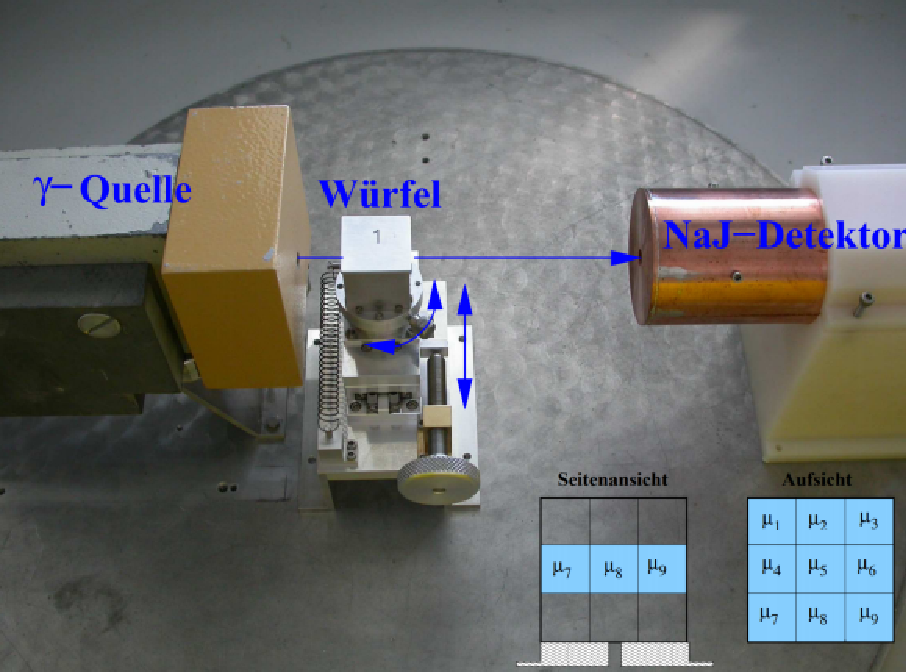
\includegraphics[width=0.8\textwidth]{figure/Aufbau.pdf}
	\caption{Auf dieser Abbildung ist der Versuchsaufbau dargestellt \cite{sample}.}
	\label{abb3}
\end{figure}

Die erste Messung wird ohne Medium durchgeführt. Die INtensität wird also für einen Zeitraum 
aufgenommen. Danach wird ein leerer Würfel aus einer Aluminiumhülle vermessen. Dafür wird 
zunächst ein Spektrum aufgenommen, bei dem die Gammastrahlung senkrecht auf einer 
Würfelfläche ein- und austritt. Danach wird der Würfel gedreht, sodass der Strahl diagonal 
durch den Würfel verläuft und daraufhin so, dass der Strahl die Nebendiagonale des 
Würfels durchquert. Die selben Messungen werden danach für zwei weitere $\SI{3}{\centi\meter} \times \SI{3}{\centi\meter}$-Würfel 
in einer Aluminiumhülle durchgeführt. Diese Würfel bestehen aus einem Innenmaterial, dass 
über die Bestimmung des Absoptionkoeffizienten ermittelt werden soll. \\\\

Für die letzte Messreihe wird ein Würfel vermessen, der verschiedene 
$\SI{1}{\centi\meter} \times \SI{1}{\centi\meter}$-Teilwürfel aus unterschiedlichem Material
enthält. Um die Teilwürfel der mittleren Ebene korrekt beschreiben zu können müssen 
zwölf Teilmessungen durchgeführt werden.
In Abbildung \ref{abb2} sind die Verläufe der Strahlung dargestellt.

\begin{figure}
	\centering
	\includegraphics[width=0.8\textwidth]{figure/Intensitäten.pdf}
	\caption{Auf dieser Abbildung sind die Verläufe der Strahlung für jede Teilmessung 
	dargestellt \cite{1}.}
	\label{abb2}
\end{figure}

Mit Hilfe der gemessenen Intensitäten können daraufhin auch für den letzten Würfel die 
Materialien bestimmt werden. Dafür muss die Matrix $A$ (siehe Kapitel \ref{sec:Absorb}) 
aufgestellt werden. Da die Teilwürfel alle Seitenlängen von 
$\SI{1}{\centi\meter}$ ist $A$ durch die Matrix 

\begin{equation}
	A = 	 
	\begin{bmatrix}
		0 		 & \sqrt{2}  & 0 		& \sqrt{2} & 0 		  & 0 		 & 0 		& 0 	   & 0\\
		0 		 & 0 		 & \sqrt{2} & 0 	   & \sqrt{2} & 0 		 & \sqrt{2} & 0 	   & 0   \\
		0 		 & 0 		 & 0 		& 0 	   & 0 		  & \sqrt{2} & 0 		& \sqrt{2} & 0 \\
		1 		 & 1 		 & 1 		& 0 	   & 0 		  & 0        & 0 		& 0 	   & 0  \\
		0 		 & 0 		 & 0 		& 1 	   & 1		  & 1		 & 0		& 0		   & 0  \\
		0 		 & 0 		 & 0 		& 0		   & 0		  & 0		 & 1		& 1		   & 1  \\
		0 		 & \sqrt{2}  & 0 		& 0		   & 0		  & \sqrt{2} & 0		& 0		   & 0 \\
		\sqrt{2} & 0 		 & 0 		& 0		   & \sqrt{2} & 0		 & 0		& 0		   & \sqrt{2} \\
		0 		 & 0 		 & 0 		& \sqrt{2} & 0		  & 0		 & 0		& \sqrt{2} & 0  \\ 
		0 		 & 0 		 & 1 		& 0		   & 0		  & 1		 & 0		& 0		   & 1\\
		0 		 & 1 		 & 0 		& 0		   & 1		  & 0		 & 0		& 1		   & 0  \\
		1 		 & 0 		 & 0 		& 1		   & 0		  & 0		 & 1		& 0		   & 0  
	\end{bmatrix}
\end{equation}

gegeben \cite{sample}.